\documentclass[12pt]{report}
\usepackage{amsmath}
\usepackage{amsfonts}
\usepackage{graphicx}


\begin{document}
Name: \hrulefill
Date: \hrulefill

\begin{center}

\bigskip
\large{\textbf{Human Variation and Disease: Discussion 1 Notes and Concept Checks}}

\bigskip
\normalsize{\textit{The goal of this discussion is to review the statistical concepts described in Appendix B described in Gillespie's ``Population Genetics: A Concise Guide'' that will be useful for this class. Questions to check conceptual understanding are provided, incorporating course material when applicable.}}

\bigskip
\normalsize{\textbf{\textit{Complete this worksheet to the best of your ability and bring it to the first discussion section. Also, please email me (leblake@uchicago.edu) any concepts or sections that you found challenging by Thursday night at midnight. }}}

\end{center}

\section{What are random variables?}

\begin{itemize}

\item A discrete random variable (e.g. \textbf{X}), is a function that takes on certain values depending on the outcome of some event, trial, or experiment.

\item An event with \textit{n} outcomes and its associated random variable may be described as follows:

\begin{tabular}{| l | c | r |}
	\hline
 Outcome & Value of \textbf{X} & Probability \\ \hline
  1 & \textit{$x_{1}$} & \textit{$p_{1}$} \\
  2 & \textit{$x_{2}$}  & \textit{$p_{2}$} \\
  3 & \textit{$x_{3}$} & \textit{$p_{3}$} \\
  . & . & . \\
  . & . & . \\
  \textit{i} & \textit{$x_{i}$}  & \textit{$p_{i}$} \\
  . & .  & . \\
  \textit{n} & \textit{$x_{n}$}  & \textit{$n_{i}$} \\ \hline
\end{tabular}

\bigskip

\item \textbf{Concept Check 1:} In the table above, what is \\ Prob \{{\textbf{X} = \textit{$x_{i}$} }\}? \hrulefill

\item \textbf{Concept Check 2:} In the table above, what is Prob \{{\textbf{X} = \textit{$x_{1}$} $\cup$ \textbf{X} = \textit{$x_{3}$}}\}? \hrulefill

\end{itemize}

\section{Moments of Random Variables}

\subsection{Mean/Expectation}

\begin{itemize}

\item The mean is a weighted average of the values taken by the random variable.

\item It is defined as \textit{E}\{\textbf{X}\} =  $\sum\limits_{i = 1}\limits^{n}$ \textit{$p_{i}$}\textit{$x_{i}$} 

\item It is often denoted by $\mu$.

\item \textbf{Concept Check 1}: Population geneticists are often interested in the mean fitness of a population, $\bar{w}$. Here, the random variable takes on the fitnesses of genotypes and the probabilities are the frequencies of those genotypes. Using the table below, write the formula for the mean fitness of a population. (For now, don't worry about the biological meanings of \textit{h} and \textit{s}.) 

\bigskip
\begin{tabular}{| l | c | r |}
	\hline
 Outcome & Value of \textbf{X} & Probability \\ \hline
  \textit{$A_{1}$$A_{1}$} & 1 & \textit{$p^{2}$} \\
  \textit{$A_{1}$$A_{2}$} & 1 - \textit{hs} & 2\textit{pq} \\
  \textit{$A_{2}$$A_{2}$} & 1- \textit{s} & \textit{$q^{2}$} \\ \hline
\end{tabular}

\bigskip

\bigskip

\bigskip

\bigskip

\bigskip

\bigskip

\bigskip

\bigskip

\textit{Note: this question is based off of the material covered in the Human Variation and Disease Lecture titled ``Selection I''}

\item \textbf{Concept Check 2}: We have measured the beaks of 5 subpopulations of finches and recorded our findings in the table below. What is the expected value of beak size for the population of finches? (In other words, what is \textit{E}\{\textbf{X}\}? Assume only these subpopulations make up the population of finches that we are interested in and there is no variation in beak length within sub-populations.) 

\bigskip
\begin{tabular}{| l | c | r |}
	\hline
 Subpopulation Number & Beak length (mm) & Subpopulation size \\ \hline
  1 & 0.4 & 100 \\
  2 & 0.55 &  300 \\
  3 & 0.65 & 150 \\ 
  4 & 0.35 &  250 \\
  5 & 0.47 & 200 \\  \hline
\end{tabular}

\bigskip

\bigskip

\bigskip

\bigskip

\bigskip

\bigskip

\bigskip

\bigskip
\textit{Note: this question is based off of the material covered in the Human Variation and Disease Lecture titled ``Quantitative Genetics I''}

\end{itemize}

\subsection{Variance}

\begin{itemize}

\item The variance of a random variable is the expectation of the squared deviations from the mean.

\item It is defined by Var\{\textbf{X}\} =  \textit{E}\{$\big (\textbf{X - $\mu$}\big)^{2}$\} = \textit{E}\{$\textbf{X}^{2}$\} -  \textit{E}\{$\textbf{X}\}^{2}$

\item It is often denoted by $\sigma^{2}$.

\item \textbf{Concept Check 3}: Using the table from the previous Concept Check, what is variance in beak size for this population of finches? (Again, assume only these subpopulations make up the population of finches that we are interested in.)

\bigskip

\bigskip

\bigskip

\bigskip

\bigskip

\bigskip

\bigskip

\bigskip
\textit{Note: this question is based off of the material covered in the Human Variation and Disease Lecture titled ``Quantitative Genetics I''}


\end{itemize}

\section{Noteworthy discrete random variables}

\subsection{Bernoulli random variable}

\begin{itemize}

\item The Bernoulli random variable is used when there is one trial of an event where there are only two possible outcomes: success (where \textbf{X} = 1) and failure (where \textbf{X} = 0). 

\item The mean of a Bernoulli random variable is \hrulefill \\
and the variance is \hrulefill.

\item \textbf{Concept Check 1}: What is a use of the Bernoulli distribution in genetics? In your example, describe what is a ``success'' and what is a '``failure''.  

\end{itemize}
\bigskip

\bigskip

\bigskip

\bigskip

\bigskip

\bigskip

\bigskip

\bigskip

\subsection{Binomial Random Variable}

\begin{itemize}

\item These random variables represent the number of success in \textit{n} independent trials when the probability of success for any one trial is \textit{p}. 

\item The random variable can take o the values 0, 1, $\ldots$, \textit{n} with probabilities

Prob \{\textbf{X} = \textit{i}\} = ${n \choose x}$ \textit{$p^{i}$} $\big( 1- \textit{p} \big)^{\textit{n-i}}$

\item \textbf{Concept Check 1}: How are Bernoulli and Binomial random variables related?

\bigskip

\bigskip

\bigskip

\item \textbf{Concept Check 2}: Keeping in mind your answer to Concept Check 2, what is the mean of a binomial random variable? The variance?

\bigskip

\bigskip

\bigskip

\item \textbf{Challenge}: In the Wright-Fisher model that we will study in class, we want to know the proportion of offspring that carry allele A from some population. What factors will be important for us to consider given that the Wright-Fisher model is a binomial sampling distribution?

\bigskip

\bigskip

\bigskip

\end{itemize}

\subsection{Poisson Random Variable}

\begin{itemize}

\item Poisson Random Variables are obtained by taking the limit of binomial random variables as \textit{n} $\rightarrow$ $\infty$ and \textit{p} $\rightarrow$ 0. 

\item Poisson random variables can take values 0, 1, $\ldots$, $\infty$ with probabilities 

Prob \{\textbf{X} = \textit{i}\} = $\frac{e^{-\mu}\mu^{i}}{i!}$

\item \textbf{Concept Check 1:} When can the Poisson distribution be used instead of the Binomial distribution? 

\bigskip

\bigskip

\bigskip
\item \textbf{Concept Check 2:} How does the Poisson distribution look different than the Binomial distribution? 

\bigskip

\bigskip

\bigskip

Overlay an example of each of the distributions on a plot below. Each distribution should have $\mu$ = 0.05 and \textit{n}= 10:

\bigskip

\bigskip

\bigskip

\bigskip

\bigskip

\bigskip

\bigskip

\bigskip

\bigskip

\bigskip

\bigskip


\item \textbf{Concept Check 3:} Would you use the Binomial or Poisson distribution to describe the distribution of crossovers along a chromosome in meiosis? Justify your answer

\end{itemize}

\bigskip

\bigskip

\bigskip

\subsection{Geometric Random Variable}

\begin{itemize}

\item The geometric random variable can take on values 1, 2, \ldots, $\infty$ describes the time until the first success in a sequence of independent trials with the probability of success, \textit{p}, and the probability of failure, \textit{q = 1-p}. 

\item Prob \{\textbf{X} = \textit{i}\} = \textit{$q^{i-1}$}\textit{p}

\item \textbf{Concept Check 1:} Why would you use the geometric distribution instead of the binomial distribution? (Hint: How are the questions answered by each different?) 

\end{itemize}

\bigskip

\bigskip

\bigskip

\section{Correlated random variables}

\begin{itemize}

\item \textbf{Concept Check 1:} If Prob\{\textbf{X} = \textit{$x_{i}$}\} = $p_{i}$ and Prob\{\textbf{Y} = $x_{i}$\} = \textit{$p_{j}$}, then the random variables \textit{X} and \textit{Y} are independent if \textit{$p_{ij}$} = \hrulefill

\item Covariance is defined as Cov \{\textbf{X,Y}\} =  \textit{E}\{\big($\textbf{X - $\mu_{x}$}$\big) \big($\textbf{Y - $\mu_{y}$}$\big)\}

\item The covariance is a measure of the tendency of two random variables to vary together. 

\bigskip
\item \textbf{Concept Check 1:} If \textit{X} and \textit{Y} tend to be large together and small together, then their covariance will be \hrulefill. 

\item If two random variables are independent, then their covariance is \hrulefill.

\item The correlation coefficient of \textit{X} and \textit{Y} = \[\frac{Cov(X, Y)}{\sqrt(Var (X))\sqrt(Var (Y))} \] 

\bigskip
\item \textbf{Concept Check 2:} In the definition of the correlation coefficient, the covariance is scaled by the variance. Why is this ``normalization'' step important? What additional information can we get from this step?

\bigskip

\bigskip

\bigskip
\item \textbf{Challenge:} Suppose we have two sites on a chromosome, \textit{A} and \textit{B}, each with two alleles in a haploid individual. If we were to plug in the probability of \textit{$A_{1}$} and \textit{$B_{1}$} into the formula for correlation coefficient, describe the information in words that we will get from this.

\bigskip

\bigskip

\bigskip
\textit{Note: These questions are based on material found in the Human Variation and Disease lectures titled ``LD'' and ``Quantative Genetics I''.}


 \end{itemize}

\bigskip

\bigskip

\bigskip
\section{Operations on random variables}

\begin{itemize}

\item If \textbf{Y} is a transformed random variable, \textbf{Y} = a\textbf{X} + b, \\ 
then \textit{E}\{\textbf{Y}\} = \textit{aE}\{\textbf{X}\} + \textit{b} and the Var\{\textbf{Y}\} = $a^{2}$Var\{\textbf{Y}\}.

\item  \textit{E}\{\textbf{X + Y}\} = \textit{E}\{\textbf{X}\} + \textit{E}\{\textbf{Y}\} regardless of whether \textit{X} and \textit{Y} and independent or dependent. \\

\item Var\{\textbf{X + Y}\} = Var\{\textbf{X}\} + Var\{\textbf{Y}\} + 2Cov\{\textbf{X + Y}\}. \\

\item \textbf{Concept Check 1:} As we can see, the variance of \{\textbf{X + Y}\} relies on the variance of \{\textbf{X}\}, the variance of \{\textbf{Y}\}, and the covariance of \{\textbf{X + Y}\}. Why do you think that is? 


\bigskip

\bigskip

\bigskip
\item \textbf{Concept Check 2:}  What is the Var\{\textbf{X + Y}\} when \textbf{X} and \textbf{Y} are independent? 

\end{itemize}

\bigskip

\bigskip

\bigskip
\section{Noteworthy continuous random variables}

\subsection{Overview}

\begin{itemize}

\item Continuous random variables can have values from -$\infty$ to $\infty$. Therefore, the probability that a continuous random variable takes on 1 particular value is \hrulefill. 

\item As a result, we will write the probability of a continuous random variable in a particular interval:

\bigskip
Prob \{\textit{a} \textless \textbf{X} \textless \textit{b} \} = $\int_{a}^{b}$ \textit{f\big(x\big) dx} \\

where \textit{f\big(x\big)} is the probability density function. 

\item \textbf{Concept Check 1:} Prob \{\textit{- $\infty$} \textless \textbf{X} \textless \textit{$\infty$} \} = $\int_{- \infty}^{\infty}$ \textit{f\big(x\big) dx} equals \hrulefill.

\end{itemize}

\subsection{Normal random variable}

\begin{itemize}

\item  \textbf{Concept Check 1:} How can you tell if a dataset is well described by the normal distribution? 

\bigskip

\bigskip

\bigskip

\item \textbf{Concept Check 2:} List some phenotypes that we might model as normally distributed:

\bigskip

\bigskip

\bigskip

\item The probability density function of the normal distribution is 
\begin{eqnarray}
\textit{f\big(x\big)} = \frac{1}{\sqrt{(2\pi)\sigma^{2}}} exp(-\frac{(x_{i}-\mu)^{2}}{2\sigma^{2}} )
\end{eqnarray}

\bigskip
\item We will often standardize a normal distribution, e.g. N(3, 10), using the transformation Z = 
$\frac{\textit{X} - \mu}{\sigma}$


\item  \textbf{Concept Check 3:} What are the advantages of ``standardizing'' a normal distribution with parameters $\mu$ and $\sigma^{2}$ so that it is N(0,1)?

\end{itemize}

\bigskip

\bigskip

\bigskip

\subsection{Beta random variable} 

\begin{itemize}

\item The Beta distribution represents a distribution of probabilities. Therefore, 0 \textless  x \textless 1.

\item If \textit{n} is a positive integer, $\Gamma$\big(\textit{n}\big) = \big(\textit{n} - 1\big)!

\item The beta random variable is distributed according to the density:

 \begin{equation} 
\textit{f\big(x\big)} = \frac{\Gamma(\alpha + \beta)x^{\alpha-1}(1-x)^{\beta-1}}{\Gamma(\alpha)\Gamma(\beta) }
\end{equation}

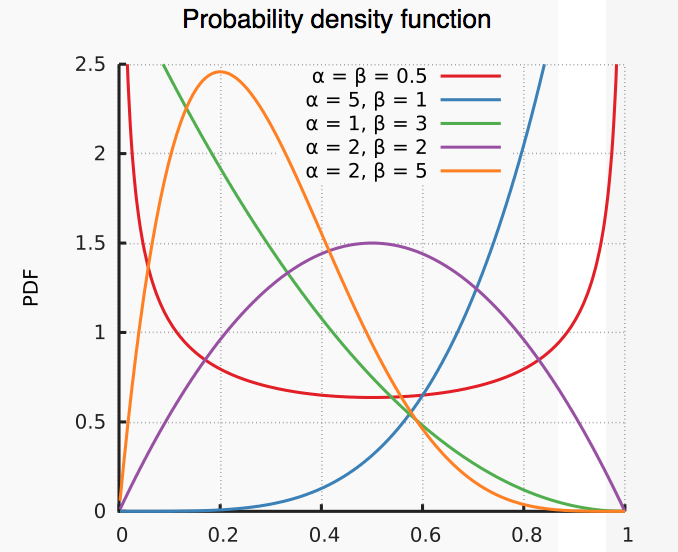
\includegraphics[width =1\textwidth]{/Users/laurenblake/Dropbox/Human_Variation_and_Disease_TA/Beta.png}

\item  \textbf{Concept Check 1:} Above are PDFs of beta distributions with different alpha and beta values. You will see that on the x-axis are probabilities. How could having a distribution of probabilities be useful in a genetics context?

\bigskip

\bigskip

\bigskip

\end{itemize}

\subsection{Bivariate normal random variable (Challenging)}

\begin{itemize}

\item We can represent two correlated random variables that each follow a normal distribution with the bivariate normal distribution. We can represent these correlated variables with random vector \textit{Z}. This vector \textit{Z} will have the vector mean $\mu$ and covarariance matrix $\Sigma$.

\item The probability density for the bivariate normal distribution Z {\raise.17ex\hbox{$\scriptstyle\sim$}} \big(X,Y\big) incorporates the means of each of the random variables (\textit{X} and \textit{Y}), the variances of the two random variables, and the correlation coefficient, $\rho$.

\[
f(x,y)=\frac{\exp \left\{ -\frac 1{2(1-\rho ^2)}\left[ \left( \frac{x-\mu _x%
}{\sigma _x}\right) ^2-2\rho \left( \frac{x-\mu _x}{\sigma _x}\right) \left( 
\frac{y-\mu _y}{\sigma _y}\right) +\left( \frac{y-\mu _y}{\sigma _y}\right)
^2\right] \right\} }{2\pi \sigma _x\sigma _y\sqrt{1-\rho ^2}} 
\]

where $(\mu _x,\mu _y)$ is the mean vector and the variance-covariance
matrix is

\[
\left( 
\begin{array}{cc}
Var(X) & Cov(X,Y) \\ 
Cov(X,Y) & Var(Y)
\end{array}
\right) =\left( 
\begin{array}{cc}
\sigma _x^2 & \rho \sigma _x\sigma _y \\ 
\rho \sigma _x\sigma _y & \sigma _y^2
\end{array}
\right) 
\]

\bigskip
\item The bivariate normal can be generalized to include more than two univariate random variables, called multivariate normal distributions. 

\item A handful of the journal articles that we read in this class will use the bivariate or multivariate normal distribution (e.g. Pritchard et al. 2000 Genetics 155:945). 

\item We will also use the moments and properties of the bivariate normal distribution, for example, in linear regression. 

\item What is the goal of linear regression? 

\newpage
\item The regression of \textbf{Y} on \textbf{X} is 


 \textit{E} \{\textbf{Y} $\mid$ \textbf{X} = x \} = $\mu_{y}$ + $\beta$ \big( \textit{x - $\mu_{x}$} \big)
 
\bigskip
where 

$\beta$ =  $\frac{Cov \{ \textbf{X},\textbf{Y} \} }{ \sigma_{x}^{2}} $

\bigskip
\textbf{Concept Check 1:} Use concepts that we have covered in this discussion and what you know about linear regression to write each of the parts of this equation in words and how it is related to linear regression. 

\bigskip  

\textit{E} \{\textbf{Y} $\mid$ \textbf{X} = x \} is 

\bigskip

\bigskip

\bigskip

$\mu_{y}$ is

\bigskip

\bigskip

\bigskip

$\beta$ is

\bigskip

\bigskip

\bigskip

 \textit{x - $\mu_{x}$} is
 
 \bigskip

\bigskip

\bigskip
 


\end{itemize}


 \bigskip

\bigskip

\bigskip

\textbf{Note:} This worksheet was created by Lauren E. Blake using the material from ``Population Genetics, A Concise Guide'' by John Gillespie 2nd edition and ``Introduction to Probability'' by D. P. Bertsekas and J. N. Tsitsiklis, 1st edition. Kindly edited by course instructor John Novembre. 




\end{document}